% Copyright 2021 Fausto Spoto
%
% Licensed under the Apache License, Version 2.0 (the "License");
% you may not use this file except in compliance with the License.
% You may obtain a copy of the License at
%
%    http://www.apache.org/licenses/LICENSE-2.0
%
% Unless required by applicable law or agreed to in writing, software
% distributed under the License is distributed on an "AS IS" BASIS,
% WITHOUT WARRANTIES OR CONDITIONS OF ANY KIND, either express or implied.
% See the License for the specific language governing permissions and
% limitations under the License.

\documentclass[11pt]{beamer}  %% versione proiettore
%%\documentclass[11pt,handout]{beamer} %% versione stampa
\usepackage{lucidiJb-2ed}
\usepackage{mathtools}
\usepackage{relsize}
\usepackage[normalem]{ulem}

\mode<article>
{
  \usepackage{fullpage}
  \usepackage{hyperref}
}

\mode<presentation>
{
  \setbeamertemplate{background canvas}[vertical shading][bottom=red!10,top=blue!10]
  \usetheme{Course}
  \usefonttheme[onlysmall]{structurebold}
}

\subtitle{Blockchain Course}
\title{Hotmoka}
\institute{Universit\`a di Verona, Italy}
\date{March 2021}

\setbeamercovered{invisible}

\def\codesize{\smaller}
\def\<#1>{\codeid{#1}}
\newcommand{\codeid}[1]{\ifmmode{\mbox{\codesize\ttfamily{#1}}}\else{\codesize\ttfamily #1}\fi}

\begin{document}

\begin{frame}
  \titlepage
\end{frame}

\begin{frame}
  \frametitle{Hotmoka}

  \begin{greenbox}{\url{https://github.com/Hotmoka/hotmoka}}
    An open-source implementation of a network of nodes:
    \begin{itemize}
    \item nodes of a blockchain
    \item IoT devices
    \item computers in the cloud
    \end{itemize}
  \end{greenbox}

  \bigskip

  \begin{greenbox}{Requests are OO-based}
    \begin{itemize}
    \item install code in the node
    \item create an object
    \item call a method of an object
    \item methods are implemented in Takamaka (subset of Java)
    \end{itemize}
  \end{greenbox}

\end{frame}

\begin{frame}\frametitle{Documentation}

  \begin{greenbox}{}
    There is an online tutorial on Hotmoka and Takamaka
    in the \<README.md> of the main repository of Hotmoka:

    \url{https://github.com/Hotmoka/hotmoka}
  \end{greenbox}

  \bigskip

  \begin{greenbox}{}
    Its examples of Takamaka projects are available here:

    \url{https://github.com/Hotmoka/hotmoka_tutorial}
  \end{greenbox}

\end{frame}

\begin{frame}\frametitle{The API of a Hotmoka node}

  \begin{itemize}
  \item \<[add|post]JarStore(request):TransactionReference>
  \item \<[add|post]ConstructorCall(request):StorageReference>
  \item \<[add|post|run]InstanceMethodCall(request):StorageValue>
  \item \<[add|post|run]StaticMethodCall(request):StorageValue>
  \item \<subscribeToEvents(key):Subscription>
  \item \<getState(StorageReference):State>
  \end{itemize}

  \bigskip

  \begin{greenbox}{}
    \<add> calls are synchronous (wait for the result)

    \smallskip
    \<post> calls are asynchronous (yield a future)

    \smallskip
    \<run> calls are synchronous and only for read-only methods
  \end{greenbox}

\end{frame}

\begin{frame}\frametitle{Nodes can be Tendermint applications}

  \begin{center}
    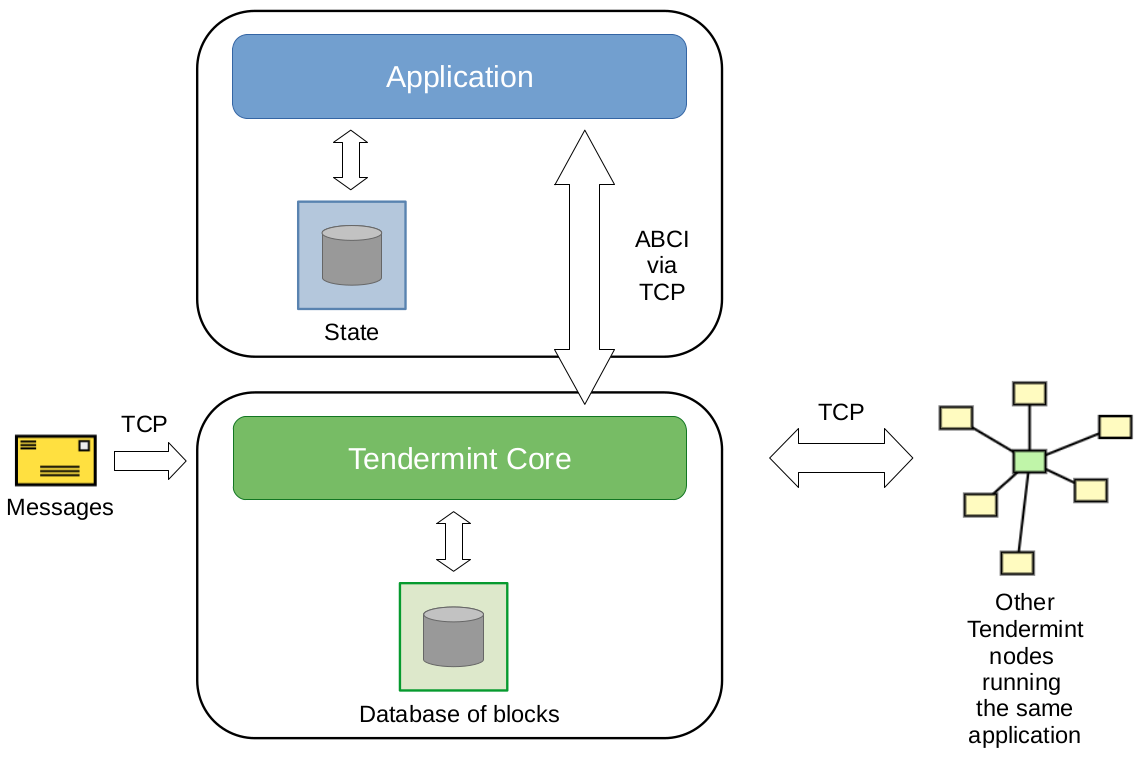
\includegraphics[width=\textwidth,clip=false]{pictures/tendermint-databases.png}
  \end{center}
    
\end{frame}

\begin{frame}\frametitle{An OO state (hash is sha256)}

  \begin{center}
    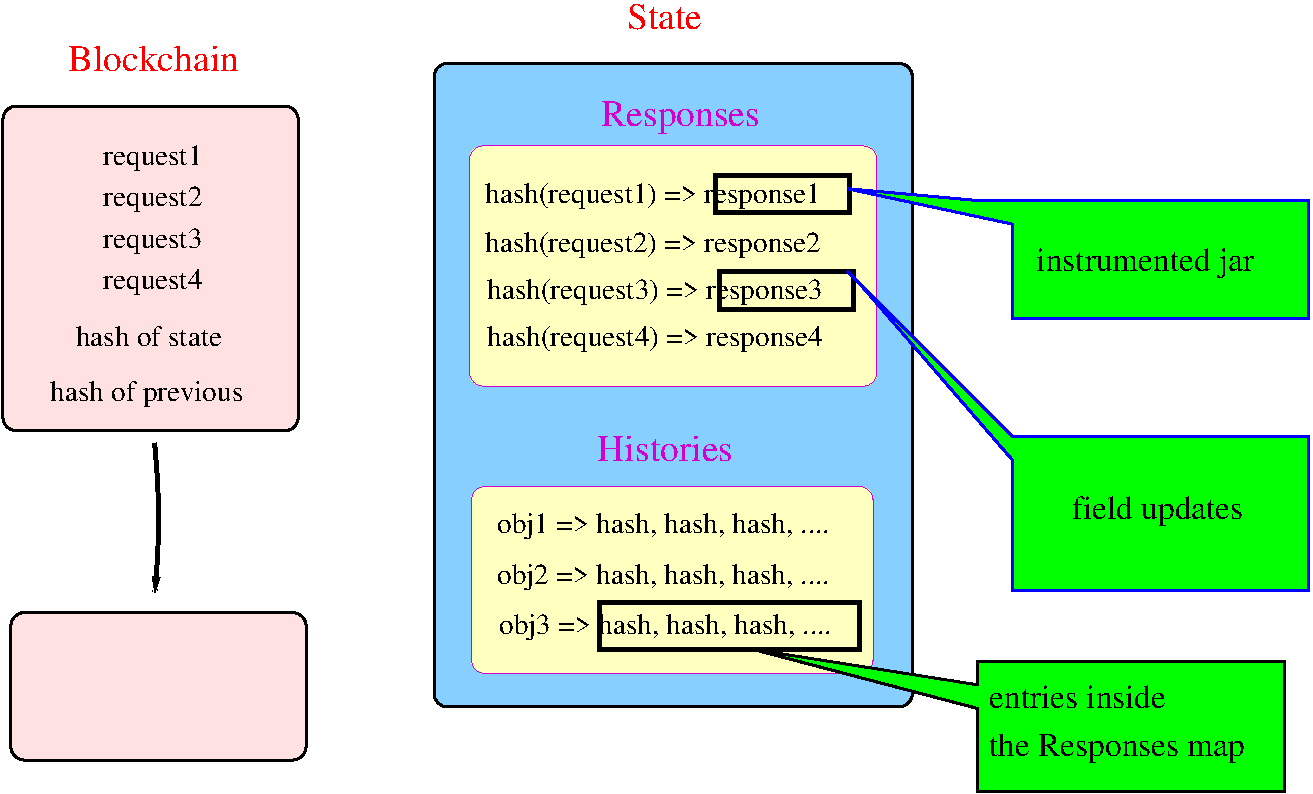
\includegraphics[width=\textwidth,clip=false]{pictures/hotmoka-structure.pdf}
  \end{center}

\end{frame}

\begin{frame}\frametitle{The API of the state}
  
    \begin{enumerate}
    \item get jar at \<hash>: access the Responses map and find the jar
    \item get object at \<obj>: access the Histories at \<obj>: for each \<hash>
      there, access the Responses map at \<hash>, project the updates on \<obj>
      and reconstruct the state of \<obj>
    \item put request/response in state: expand Responses with hash(request)$\Rightarrow$response
      \begin{itemize}
      \item[] if the response contains updates, add hash(request) to the histories of
        the updated objects
      \end{itemize}
    \item \<h=get\_hash()>: compute the hash of the hash of the Merkle-Patricia trie for
      Responses and of that for Histories
    \item \sout{\<checkout(h)>} $\Rightarrow$ unused data from points above are garbage-collected
    \end{enumerate}

\end{frame}

\begin{frame}[fragile]\frametitle{Start experimenting with Hotmoka$^*$}

  \begin{enumerate}
  \item ensure to have Java version $\ge$ 11 installed

  \item ensure to have git and Maven installed

  \item download Hotmoka

    {\color{blue}\<git clone https://github.com/Hotmoka/hotmoka.git -b univr>}

  \item let Maven compile and install it in your local Maven repository

    {\color{blue}\<mvn clean install -DskipTests>}

  \end{enumerate}


  \bigskip
  \bigskip
  \bigskip
  \bigskip
  \bigskip
  \bigskip
  {\tiny $^*$ The network server used in the experiment is joint work with Dinu Berinde}

\end{frame}

% How I started the node:
%java --module-path modules/explicit:modules/automatic --class-path "modules/unnamed/*" --module io.hotmoka.tools/io.hotmoka.tools.Moka init-tendermint 1000000000000000000000000000000000000 --open-unsigned-faucet

\begin{frame}[fragile]\frametitle{Info about a Hotmoka node}

  A Hotmoka node over Tendermint has been published on AWS for the duration of this course

  \bigskip

  \begin{greenbox}{Run this inside the Hotmoka repository (on a single line!)}
    {\small\begin{semiverbatim}
java {\color{red}--module-path modules/explicit:modules/automatic
     --class-path "modules/unnamed/*"}
     {\color{blue}--module io.hotmoka.tools/io.hotmoka.tools.Moka} info
     --url panarea.hotmoka.io
    \end{semiverbatim}}
  \end{greenbox}

  \medskip

  \begin{greenbox}{You can define an alias to simplify the command (single line!)}
    {\small\begin{semiverbatim}
alias Moka='java --module-path modules/explicit:modules/automatic
                --class-path "modules/unnamed/*"
                --module io.hotmoka.tools/io.hotmoka.tools.Moka'
    \end{semiverbatim}}
  \end{greenbox}

  \medskip

  \begin{greenbox}{Use the alias instead}
{\small\<Moka info --url panarea.hotmoka.io>}
  \end{greenbox}

\end{frame}

\begin{frame}[fragile]\frametitle{\<Moka info --url panarea.hotmoka.io>}

{\tiny\begin{semiverbatim}
 {\color{red}takamakaCode:} 02dfd29348abaa44f720525179fa170f26063c973fd40c3ff368a9402551882c
 {\color{red}manifest:} 42a8a11aee0405aee5775514b3b0456c7740bbb015b4b87df4776e6e4add7668#0
   chainId: {\color{violet}chain-ASdWiN}
   maxErrorLength: 300
   maxDependencies: 20
   maxCumulativeSizeOfDependencies: 10000000
   allowsSelfCharged: false
   {\color{violet}allowsUnsignedFaucet: true}
   skipsVerification: false
   signature: ed25519
   {\color{red}gamete:} 4f7d7ca1fbea152d8f323c21e1abcfa1d979c7c4ea667d8457381a26b08a2d71#0
     balance: 999999999999999999999999999999992180
     redBalance: 0
     {\color{violet}maxFaucet: 1000000}
     maxRedFaucet: 0
   {\color{red}gasStation:} 42a8a11aee0405aee5775514b3b0456c7740bbb015b4b87df4776e6e4add7668#10
     {\color{violet}gasPrice: 1}
     maxGasPerTransaction: 1000000000
     ignoresGasPrice: false
     targetGasAtReward: 1000000
     inflation: 10000 (ie. 0.10%)
     oblivion: 250000 (ie. 25.00%)
   {\color{red}validators:} 42a8a11aee0405aee5775514b3b0456c7740bbb015b4b87df4776e6e4add7668#2
     {\color{violet}number of validators: 1}
     validator #0: 42a8a11aee0405aee5775514b3b0456c7740bbb015b4b87df4776e6e4add7668#1
       id: C220489CDBAE0FAFF8F8286A9C541FD55BA2CE7C 
       power: 1
     ticketForNewPoll: 100
     number of polls: 0
   {\color{red}versions:} 42a8a11aee0405aee5775514b3b0456c7740bbb015b4b87df4776e6e4add7668#f
     verificationVersion: 0
  \end{semiverbatim}}

\end{frame}

\begin{frame}\frametitle{The minimal content of a Hotmoka node's state}

  \begin{center}
    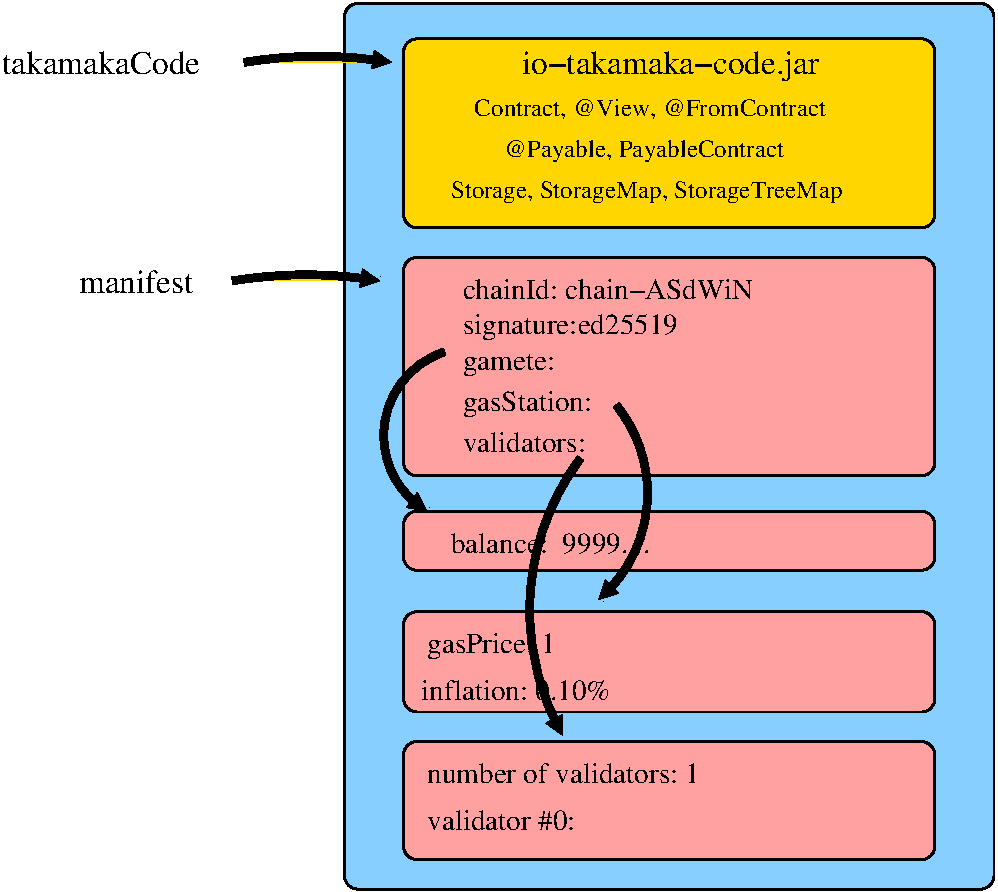
\includegraphics[scale=0.5,clip=false]{pictures/state1.pdf}
  \end{center}
  
\end{frame}

\begin{frame}[fragile]\frametitle{The state contains actual Java objects}

  {\scriptsize
    \texttt{manifest:} $\underbrace{{\color{red}\mathtt{42a8a11aee0405aee5775514b3b0456c7740bbb015b4b87df4776e6e4add7668\#0}}}_{\text{machine-independent memory address of an object}}$
  }

  \bigskip

  \begin{greenbox}{{\scriptsize\<Moka state 42a8a11aee0405aee5775514b3b0456c7740bbb015b4b87df4776e6e4add7668\#0 --url panarea.hotmoka.io>}}
    {\tiny\begin{semiverbatim}
class {\color{violet}io.takamaka.code.governance.Manifest} (from jar installed at 02dfd29348abaa44f7205251...)
  allowsSelfCharged:boolean = false
  allowsUnsignedFaucet:boolean = true
  chainId:java.lang.String = "chain-ASdWiN"
  gamete:io.takamaka.code.lang.Account = {\color{red}4f7d7ca1fbea152d8f323c21e1abcfa1d979c7c4ea667d8457381a26b08a2d71#0}
  gasStation:io.takamaka.code.governance.GasStation = {\color{red}42a8a11aee0405aee5775514b3b0456c7740bbb015b4b8...}
  maxCumulativeSizeOfDependencies:long = 10000000
  maxDependencies:int = 20
  maxErrorLength:int = 300
  signature:java.lang.String = "ed25519"
  skipsVerification:boolean = false
  validators:io.takamaka.code.governance.Validators = {\color{red}42a8a11aee0405aee5775514b3b0456c7740bbb015b4b8...}
  versions:io.takamaka.code.governance.Versions = {\color{red}42a8a11aee0405aee5775514b3b0456c7740bbb015b4b87df4...}
^ balance:java.math.BigInteger = 0 {\color{violet}(inherited from io.takamaka.code.lang.Contract)}
^ balanceRed:java.math.BigInteger = 0 {\color{violet}(inherited from io.takamaka.code.lang.Contract)}
^ nonce:java.math.BigInteger = 227 {\color{violet}(inherited from io.takamaka.code.lang.ExternallyOwnedAccount)}
^ publicKey:java.lang.String = "" {\color{violet}(inherited from io.takamaka.code.lang.ExternallyOwnedAccount)}
    \end{semiverbatim}}
  \end{greenbox}

\end{frame}

\begin{frame}[fragile]\frametitle{Creation of a new account}

  Let us create a new account with 50000000 units of coin:

  \smallskip

  \begin{greenbox}{{\small\<Moka create-account 50000000 --payer faucet --url panarea.hotmoka.io>}}
    {\tiny\begin{semiverbatim}
Free account creation will succeed only if the gamete of the node supports an open unsigned faucet
{\color{armygreen}total gas consumed: 49392}
{\color{darkred}  for CPU: 601
  for RAM: 1478
  for storage: 47313
  for penalty: 0}
A new account 06aa6a1afabc82c7161ffcdc2391a2136101aaeb94f64edd53a1d0d1436d610e\#0 has been created
{\color{blue}The keys of the account have been saved
  into the file 06aa6a1afabc82c7161ffcdc2391a2136101aaeb94f64edd53a1d0d1436d610e\#0.keys}
    \end{semiverbatim}}
  \end{greenbox}

  \bigskip

  \begin{redbox}{Who paid for that?}
    Gas and coins have been paid by the gamete, then provides an unsigned \emph{faucet}.
    This is a testnet. A real network has no open unsigned faucet
    and one must specify the address of the payer account then
    (with \<--payer>)
  \end{redbox}

\end{frame}

\begin{frame}[fragile]\frametitle{Let us have a look at our first account}

    \begin{greenbox}{{\scriptsize\<Moka state 06aa6a1afabc82c7161ffcdc2391a2136101aaeb94f64edd53a1d0d1436d610e\#0 --url panarea.hotmoka.io>}}
    {\tiny\begin{semiverbatim}
class {\color{violet}io.takamaka.code.lang.ExternallyOwnedAccount} (from jar installed at 02dfd29348abaa...)
  nonce:java.math.BigInteger = 0
  publicKey:java.lang.String = "MCowBQYDK2VwAyEAk45GxqvRFg88bKZqkqDGxQBHdvvZF+b9YSkl8xs28Ao="
^ balance:java.math.BigInteger = 50000000 (inherited from io.takamaka.code.lang.Contract)
^ balanceRed:java.math.BigInteger = 0 (inherited from io.takamaka.code.lang.Contract)
    \end{semiverbatim}}
  \end{greenbox}

  \bigskip

  \begin{itemize}
  \item the nonce starts from 0
  \item the initial balance is actually 50000000
  \item the public key is a Base64-encoded ed25519 key
  \item the public key is stored in the object: no need to send it again at every future
    method call (like Ethereum does instead)
  \end{itemize}

\end{frame}

\begin{frame}\frametitle{A new object in state}

  \begin{center}
    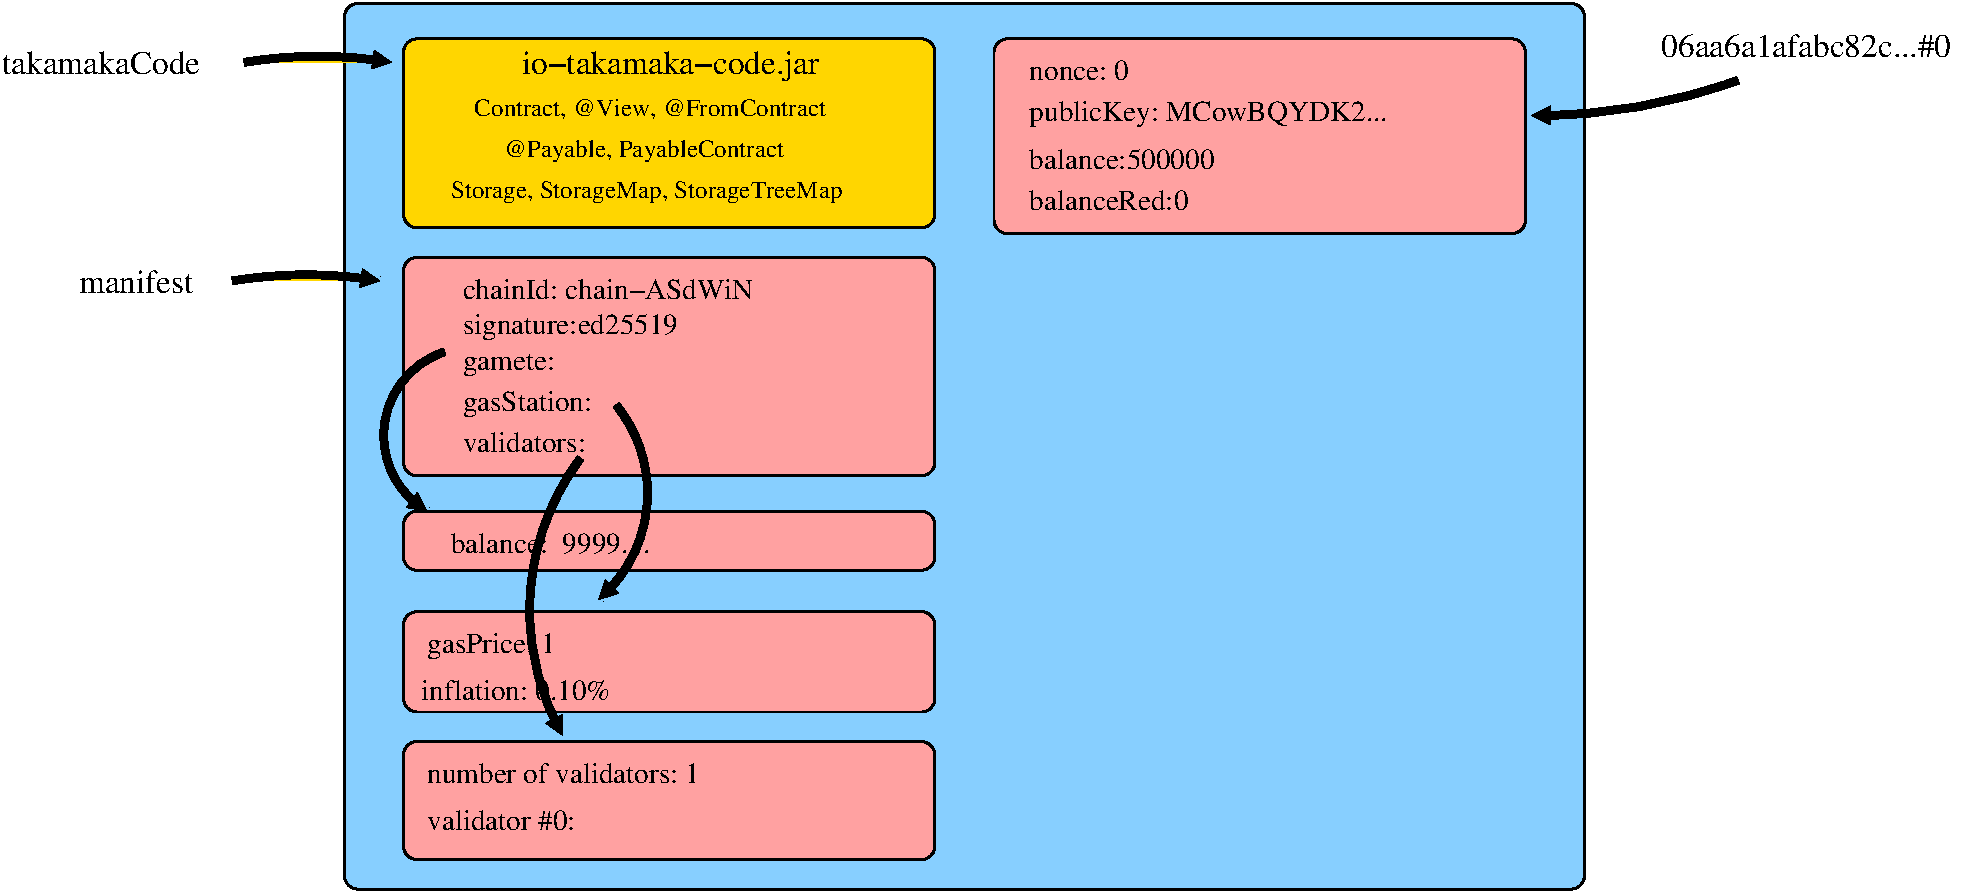
\includegraphics[scale=0.37,clip=false]{pictures/state2.pdf}
  \end{center}
  
\end{frame}

\begin{frame}[fragile]\frametitle{Let us have a look at the API of our first account}

    \begin{greenbox}{{\scriptsize\<Moka state 06aa6a1afabc82c7161ffcdc2391a2136101aaeb94f64edd53a1d0d1436d610e\#0 {\color{orange}--api} --url panarea.hotmoka.io>}}
    {\tiny\begin{semiverbatim}
class {\color{violet}io.takamaka.code.lang.ExternallyOwnedAccount} (from jar installed at 02dfd29348abaa...)
  nonce:java.math.BigInteger = 0
  publicKey:java.lang.String = "MCowBQYDK2VwAyEAk45GxqvRFg88bKZqkqDGxQBHdvvZF+b9YSkl8xs28Ao="
^ balance:java.math.BigInteger = 50000000 (inherited from io.takamaka.code.lang.Contract)
^ balanceRed:java.math.BigInteger = 0 (inherited from io.takamaka.code.lang.Contract)

  {\color{red}@Payable @FromContract} public ExternallyOwnedAccount(java.math.BigInteger,java.lang.String)
  {\color{red}@Payable @FromContract} public ExternallyOwnedAccount(long,java.lang.String)
  {\color{red}@Payable @FromContract} public ExternallyOwnedAccount(int,java.lang.String)
  public ExternallyOwnedAccount(java.lang.String)

  {\color{red}@View} public final java.math.BigInteger nonce()
  {\color{red}@View} public final java.lang.String publicKey()
  {\color{red}@View} public java.lang.String toString()
^ {\color{red}@View} public final java.math.BigInteger balance() (inherited from io.takamaka.code.lang.Contract)
^ {\color{red}@View} public final java.math.BigInteger balanceGreen() (inherited from io.takamaka.code.lang.Contract)
^ {\color{red}@View} public final java.math.BigInteger balanceRed() (inherited from io.takamaka.code.lang.Contract)
^ public final int compareByStorageReference(io.takamaka.code.lang.Storage)
    (inherited from io.takamaka.code.lang.Storage)
^ public boolean equals(java.lang.Object) (inherited from java.lang.Object)
^ public final native java.lang.Class getClass() (inherited from java.lang.Object)
^ {\color{red}@View} public final java.lang.String getClassName() (inherited from io.takamaka.code.lang.Storage)
^ public native int hashCode() (inherited from java.lang.Object)
^ {\sout{public final native void notify() (inherited from java.lang.Object)}} {\color{red}X}
^ {\sout{public final native void notifyAll() (inherited from java.lang.Object)}} {\color{red}X}
^ {\color{red}@Payable @FromContract} public final void receive(int)
    (inherited from io.takamaka.code.lang.PayableContract)
^ {\color{red}@Payable @FromContract} public final void receive(java.math.BigInteger)
    (inherited from io.takamaka.code.lang.PayableContract)
  ...
    \end{semiverbatim}}
  \end{greenbox}

\end{frame}

\begin{frame}[fragile]\frametitle{Let us call \<toString()> on our first account}

\begin{tt}
Moka call <payer> <receiver> <methodName> [<args>...]
\end{tt}

\bigskip

We will use our account as payer and as receiver at the same time:

\bigskip

\begin{greenbox}{{\small\<Moka call 06aa6a1afabc82c7161ffcdc2391a2136101aaeb94f64edd53a1d0d1436d610e\#0 06aa6a1afabc82c7161ffcdc2391a2136101aaeb94f64edd53a1d0d1436d610e\#0 toString --url panarea.hotmoka.io>}}
    {\begin{semiverbatim}
{\color{blue}an externally owned account}
calls to @View methods consume no gas 
    \end{semiverbatim}}
  \end{greenbox}

\bigskip

\begin{center}
  \<toString()> in class \<ExternallyOwnedAccount> is annotated as \<@View>
\end{center}

\end{frame}

\begin{frame}\frametitle{The execution of a method (or constructor)}

  \begin{greenbox}{The request specifies}
    \begin{itemize}
    \item payer object, receiver object and actual arguments (\emph{input})
    \item classpath, signature of the method
    \item nonce, chain id, gas price, gas limit
    \item signature of the request
    \end{itemize}
  \end{greenbox}

  \bigskip

  \begin{greenbox}{The computation of the response (ie, the execution of the request)}
    \begin{enumerate}
    \item create a classloader form the jar(s) in state for the classpath
    \item reconstruct, from the state, RAM objects for \emph{input}
    \item execute the method on a normal Java Virtual Machine (in RAM)
    \item at the end, identify updates to fields of objects reachable from \emph{input}
      or return value
    \item pack those updates into a response (RAM objects destroyed now)
    \item put request/response in state, expanding histories
    \end{enumerate}
  \end{greenbox}

\end{frame}

\begin{frame}[fragile]\frametitle{How can Hotmoka identify updates to fields of objects?}

  \begin{greenbox}{The original code}
    \begin{semiverbatim}
      public class C \{
        public {\color{blue}int i;}
        public void foo() \{
          {\color{blue}i} = 42;
        \}
      \}
    \end{semiverbatim}
  \end{greenbox}

  \begin{center}
    No way to know if \<i> changed its value during the execution of \<foo()>
  \end{center}

\end{frame}

\begin{frame}[fragile]\frametitle{How can Hotmoka identify updates to fields of objects?}

  \begin{greenbox}{The instrumented code}
    \begin{semiverbatim}
      public class C {\color{red}extends Storage} \{
        public {\color{blue}int i, old\_i;} // aliased at method start
        public void foo() \{
          {\color{blue}i} = 42;
        \}
      \}
    \end{semiverbatim}
  \end{greenbox}

  \begin{center}
    \<i> changed its value during the execution of \<foo()> iff at the end \<i>$\not=$\<old\_i>
  \end{center}

\end{frame}

\begin{frame}[fragile]\frametitle{How can Hotmoka enforce gas limits?}

  \begin{greenbox}{The original code}
    \begin{semiverbatim}
      public class C \{
        public void foo() \{
          while (...) \{
            ...
          \}
        \}
      \}
    \end{semiverbatim}
  \end{greenbox}

  \begin{center}
    This loop might run for very long or even forever
  \end{center}

\end{frame}

\begin{frame}[fragile]\frametitle{How can Hotmoka enforce gas limits?}

  \begin{greenbox}{The instrumented code}
    \begin{semiverbatim}
      {\color{blue}static long counter;}
      public class C \{
        public void foo() \{
          while (...) \{
            {\color{blue}if (counter++ >= gaslimit)
              throw new OutOfGasError();}
            ...
          \}
        \}
      \}
    \end{semiverbatim}
  \end{greenbox}

  \begin{center}
    Actual gas costs are more fine-grained
  \end{center}

\end{frame}

\begin{frame}\frametitle{Verification and instrumentation of jars in state}

  Each jar that gets installed in a Hotmoka node undergoes two processes:

  \begin{enumerate}
  \item Verification: absence of frequent errors
    \begin{itemize}
    \item objects stored in state extend \<Storage>
    \item non-deterministic or non-terminating library code is not used
    \item no synchronization
    \item no native code
    \item no \emph{dangerous} bytecodes
    \item no finalizers
    \item no static fields (mostly)
    \item code annotations are used correctly
    \item \ldots
    \end{itemize}
  \item Instrumentation
    \begin{itemize}
    \item fields of \<Storage> classes get duplicated
    \item gas metering is weaved into the code
    \item code annotations get implemented \emph{by magic}
    \item \ldots
    \end{itemize}
  \end{enumerate}

\end{frame}

\begin{frame}\frametitle{The Takamaka programming language}

  Takamaka is the subset of Java that passes the verification
  of a Hotmoka node. It uses code annotations to implement contract-based aspects:

  \begin{itemize}
  \item {\color{blue}\<@FromContract>} annotates something that can only be called by a contract,
    not by any other code; hence, it has a {\color{blue}\<caller()>}
  \item {\color{blue}\<@Payable>} annotates something whose execution requires to pay some
    cryptocurrency units
  \item {\color{blue}\<@View>} annotates something whose execution can be run for free,
    without paying for its gas: it must not generate any update at its end
    (\emph{pure} code)
  \end{itemize}

  \bigskip
  Takamaka comes equipped with a {\color{blue}support library}
  (\<io-takamaka-code>) that defines such annotations and
  other typical classes that are useful
  for programming smart contracts

\end{frame}

\begin{frame}[fragile]\frametitle{A first example of Takamaka code}

  \begin{enumerate}
  \item create a new Java Maven project (skip archetype selection)
  \item edit the Maven configuration file \<pom.xml> as follows:
\vspace*{-1ex}{\tiny\begin{semiverbatim}
{\color{blue}{
<project ...>
  <modelVersion>4.0.0</modelVersion>

  {\color{armygreen}<groupId>io.hotmoka</groupId>
  <artifactId>ponzi</artifactId>
  <version>0.0.1</version>}

  {\color{violet}{<properties>
    <project.build.sourceEncoding>UTF-8</project.build.sourceEncoding>
    <maven.compiler.source>11</maven.compiler.source>
    <maven.compiler.target>11</maven.compiler.target>
    <failOnMissingWebXml>false</failOnMissingWebXml>
  </properties>}}

  {\color{red}{<dependencies> <dependency>
      <groupId>io.hotmoka</groupId>
      <artifactId>io-takamaka-code</artifactId>
      <version>1.0.0</version>
  </dependency> </dependencies>}}

  {\color{violet}{<build> <plugins> <plugin>
        <groupId>org.apache.maven.plugins</groupId>
        <artifactId>maven-compiler-plugin</artifactId>
        <version>3.8.1</version>
        <configuration> <release>11</release> </configuration>
  </plugin> </plugins> </build>}}

</project>
}}\end{semiverbatim}}
  \end{enumerate}

\end{frame}

\begin{frame}[fragile]\frametitle{A first example of Takamaka code}

  \begin{enumerate}
    \setcounter{enumi}{2}
  \item create a source package \<io.takamaka.ponzi> inside \<src/main/java>
  \item create a \<module-info.java> in the \<src/main/java> directory:
    \vspace*{-3ex}\begin{semiverbatim}
{\color{blue}{
module ponzi \{
  requires io.takamaka.code;
\}
}}\end{semiverbatim}
  \end{enumerate}

\end{frame}

\begin{frame}[fragile]\frametitle{A first example of Takamaka code}

  \begin{enumerate}
    \setcounter{enumi}{4}
      \item add the following class in package \<io.takamaka.ponzi>
\vspace*{-1ex}{\tiny\begin{semiverbatim}
{\color{darkblue}{
package io.takamaka.ponzi;

import static io.takamaka.code.lang.Takamaka.require;
import java.math.BigInteger;
import io.takamaka.code.lang.Contract;
import io.takamaka.code.lang.FromContract;
import io.takamaka.code.lang.Payable;
import io.takamaka.code.lang.PayableContract;
import io.takamaka.code.lang.View;

public class SimplePonzi {\color{red}extends Contract} \{
  private final BigInteger _10 = BigInteger.valueOf(10L), _11 = BigInteger.valueOf(11L);
  private {\color{armygreen}PayableContract} currentInvestor;
  private BigInteger currentInvestment = BigInteger.ZERO;

  public {\color{violet}@Payable} {\color{armygreen}@FromContract(PayableContract.class)} void invest({\color{violet}BigInteger amount}) \{
    BigInteger minimum = currentInvestment.multiply(_11).divide(_10);
    require(amount.compareTo(minimum) >= 0, () -> "you must invest at least " + minimum);

    if (currentInvestor != null)
      currentInvestor.{\color{armygreen}receive(amount)}; {\color{red}// no risk of reentrancy}

    currentInvestor = {\color{armygreen}(PayableContract) caller()};
    currentInvestment = amount;
  \}

  public {\color{red}@View} BigInteger getCurrentInvestment() \{
    return currentInvestment;
  \}
\}
}}\end{semiverbatim}}
  \end{enumerate}

\end{frame}

\begin{frame}[fragile]\frametitle{A first example of Takamaka code}

  \begin{enumerate}
    \setcounter{enumi}{5}
  \item compile and package everything with Maven:

    {\color{blue}\<mvn package>}

  \item the compiled \<ponzi-0.0.1.jar> will appear inside the
    \<target> directory of your project, ready to be installed in a
    Hotmoka node

  \item install \<ponzi-0.0.1.jar> in our AWS Hotmoka node (\begin{tt}Moka install <payer> <jar>\end{tt})
  \end{enumerate}

  \medskip

  \begin{greenbox}{}
    {\color{armygreen}\scriptsize{\begin{tt}
          Moka install

          06aa6a1afabc82c7161ffcdc2391a2136101aaeb94f64edd53a1d0d1436d610e\#0

          .../target/ponzi-0.0.1.jar

          --url panarea.hotmoka.io
    \end{tt}}}
    {\scriptsize\begin{semiverbatim}
Do you really want to spend up to 443300 gas units to install the jar [Y/N] Y
.../target/ponzi-0.0.1.jar has been installed at
  {\color{red}39f999a63555542eaf5040388d61c20193dee4fb035847a40608c494bf069765}
{\color{armygreen}total gas consumed: 298189}
{\color{darkred}  for CPU: 233
  for RAM: 1164
  for storage: 296792
  for penalty: 0}
    \end{semiverbatim}}
  \end{greenbox}

\end{frame}

\begin{frame}\frametitle{A new jar in state}

  \begin{center}
    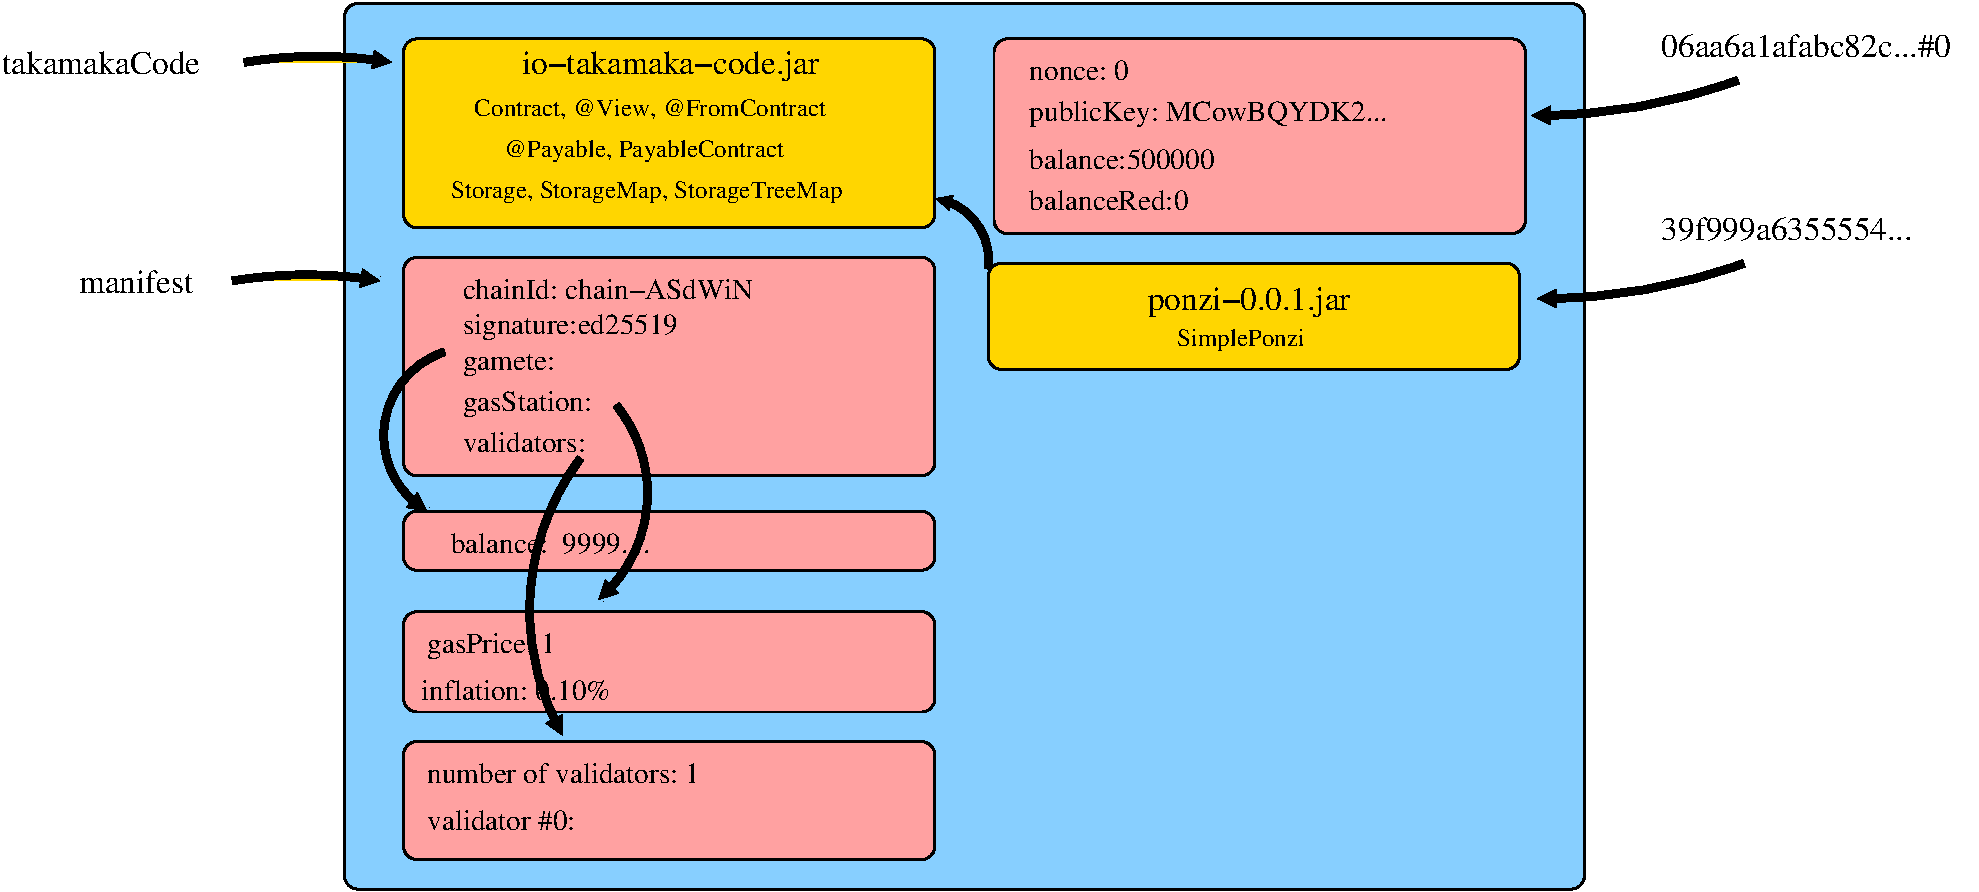
\includegraphics[scale=0.37,clip=false]{pictures/state3.pdf}
  \end{center}
  
\end{frame}

\begin{frame}[fragile]\frametitle{Creation of a new object in state}

\begin{tt}
Moka create <payer> <className> [<args>...]
\end{tt}

\bigskip

We use our account as payer and specify where \<SimplePonzi> is defined
(the \alert{classpath}):

\bigskip

\begin{greenbox}{}
    {\color{armygreen}\scriptsize{\begin{tt}
          Moka create

          06aa6a1afabc82c7161ffcdc2391a2136101aaeb94f64edd53a1d0d1436d610e\#0

          io.takamaka.ponzi.SimplePonzi

          --classpath 39f999a63555542eaf5040388d61c20193dee4fb035847a40608c494bf069765

          --url panarea.hotmoka.io
    \end{tt}}}
    {\tiny\begin{semiverbatim}
do you really want to spend up to 500000 gas units to call {\color{red}public SimplePonzi()} ? [Y/N] Y
the new object has been allocated at 754371b03ef2c413f546e1c3667adf86d545a3587e60f75d2c496863ef442f5c\#0
{\color{armygreen}total gas consumed: 42686}
{\color{darkred}  for CPU: 280
  for RAM: 1113
  for storage: 41293
  for penalty: 0}
    \end{semiverbatim}}
  \end{greenbox}

\end{frame}

\begin{frame}\frametitle{A new \<SimplePonzi> in state}

  \begin{center}
    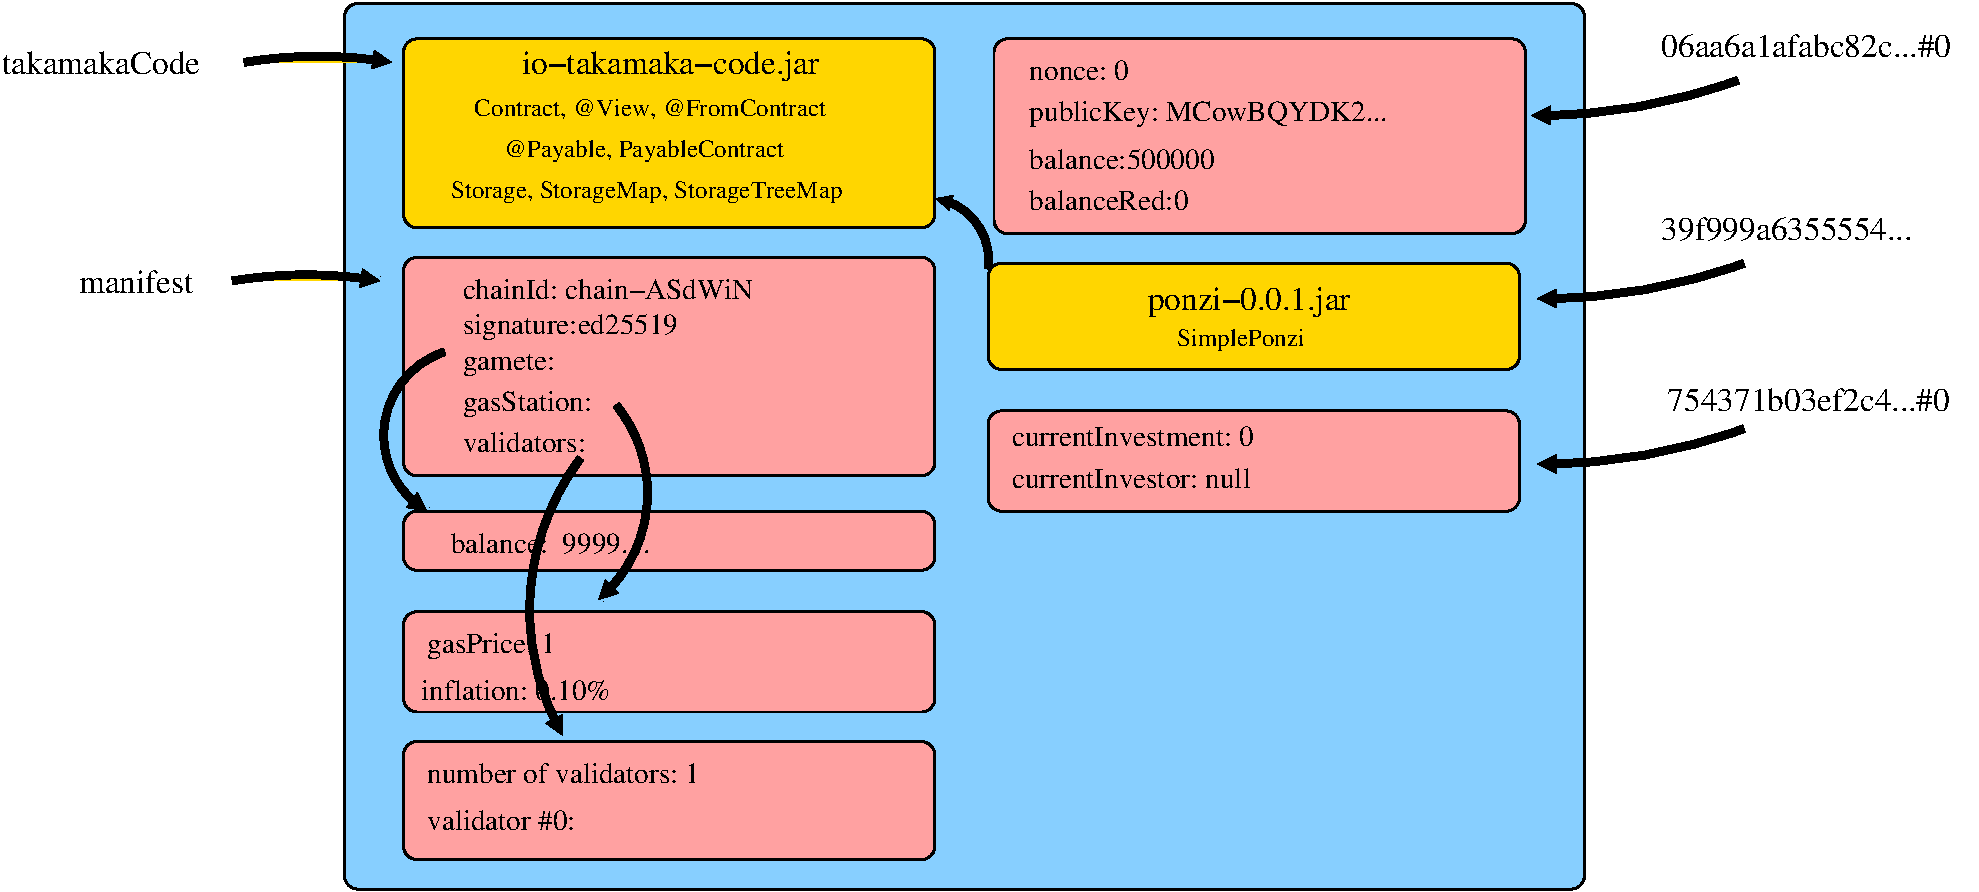
\includegraphics[scale=0.37,clip=false]{pictures/state4.pdf}
  \end{center}
  
\end{frame}

\begin{frame}[fragile]\frametitle{Call the \<invest> method of our contract}

\begin{tt}
Moka call <payer> <receiver> <methodName> [<args>...]
\end{tt}

\medskip

We use our account as payer:

\medskip

\begin{greenbox}{}
 {\color{armygreen}\scriptsize{\begin{tt}
          Moka call

          06aa6a1afabc82c7161ffcdc2391a2136101aaeb94f64edd53a1d0d1436d610e\#0

          754371b03ef2c413f546e1c3667adf86d545a3587e60f75d2c496863ef442f5c\#0

          invest

          40000

          --url panarea.hotmoka.io
 \end{tt}}}
 {\tiny\begin{semiverbatim}
Do you really want to spend up to 500000 gas units to call
  {\color{red}@Payable @FromContract(PayableContract.class) public void invest(java.math.BigInteger)} ? [Y/N] Y
{\color{armygreen}total gas consumed: 10373}
{\color{darkred}  for CPU: 402
  for RAM: 1253
  for storage: 8718
  for penalty: 0}
    \end{semiverbatim}}
  \end{greenbox}

\end{frame}

\begin{frame}[fragile]\frametitle{Call the \<invest> method of our contract, again}

\begin{tt}
Moka call <payer> <receiver> <methodName> [<args>...]
\end{tt}

\medskip

We use our account as payer:

\medskip

\begin{greenbox}{}
 {\color{armygreen}\scriptsize{\begin{tt}
          Moka call

          06aa6a1afabc82c7161ffcdc2391a2136101aaeb94f64edd53a1d0d1436d610e\#0

          754371b03ef2c413f546e1c3667adf86d545a3587e60f75d2c496863ef442f5c\#0

          invest

          40000

          --url panarea.hotmoka.io
 \end{tt}}}
    {\tiny\begin{semiverbatim}
Do you really want to spend up to 500000 gas units to call
  {\color{red}@Payable @FromContract(PayableContract.class) public void invest(java.math.BigInteger)} ? [Y/N] Y
{\color{armygreen}total gas consumed: 500000}
{\color{darkred}  for CPU: 446
  for RAM: 1353
  for storage: 8718
  for penalty: 489483}
{\color{red}io.hotmoka.beans.TransactionException: io.takamaka.code.lang.RequirementViolationException:
  you must invest at least 44000@SimplePonzi.java:18}
\end{semiverbatim}}
\end{greenbox}

\end{frame}

\begin{frame}[fragile]\frametitle{A gradual Ponzi scheme}

{\tiny\begin{semiverbatim}
package io.hotmoka.examples.ponzi;

import static io.takamaka.code.lang.Takamaka.require;

import java.math.BigInteger;
import io.takamaka.code.lang.Contract;
import io.takamaka.code.lang.FromContract;
import io.takamaka.code.lang.Payable;
import io.takamaka.code.lang.PayableContract;
import io.takamaka.code.util.StorageList;
import io.takamaka.code.util.StorageLinkedList;

public class GradualPonzi extends Contract \{
  private final BigInteger MINIMUM = BigInteger.valueOf(1_000L);
  private final {\color{red}StorageList<PayableContract> investors = new StorageLinkedList<>();}

  public {\color{violet}@FromContract(PayableContract.class)} GradualPonzi() \{
    investors.add({\color{violet}(PayableContract) caller()});
  \}

  public {\color{airforceblue}@Payable} {\color{violet}@FromContract(PayableContract.class)} void invest({\color{airforceblue}BigInteger amount}) \{
    require(amount.compareTo(MINIMUM) >= 0, () -> "you must invest at least " + MINIMUM);
    BigInteger eachInvestorGets = amount.divide(BigInteger.valueOf(investors.size()));
    investors.stream().forEachOrdered(investor -> investor.receive(eachInvestorGets));
    investors.add({\color{violet}(PayableContract) caller()});
  \}
\}
\end{semiverbatim}}

\end{frame}

\begin{frame}[fragile]\frametitle{An insurance contract}

  \begin{greenbox}{The contract allows one to insure specific days of the year}
    If it rains on those days, one will get an indemnization larger than
    the cost of the insurance
    \begin{itemize}
    \item much larger in summer
    \item just a bit larger in winter
    \end{itemize}
  \end{greenbox}

  \medskip
  The contract provides the following functionalities:

  \begin{itemize}
  \item construction, upon specification of the oracle:
    \[\<{\color{violet}@FromContract} {\color{airforceblue}@Payable} Insurance({\color{airforceblue}BigInteger amount}, Contract oracle)>\]
  \item purchase of an insurance for specific days:
    \[\<{\color{violet}@FromContract(PayableContract.class)} {\color{airforceblue}@Payable} void buy>\]
    \vspace*{-5ex}
    \[\<({\color{airforceblue}long amount}, int day, int month, int year, int duration)>\]
  \item notification of rain and indemnization:
    \[\<{\color{violet}@FromContract} void itRains()>\]
  \end{itemize}
\end{frame}

\begin{frame}[fragile]\frametitle{An insurance contract}

  {\scriptsize\begin{semiverbatim}
public class Insurance extends {\color{blue}Contract} \{
  public final static long MIN = 1_000, MAX = 1_000_000_000;
  private final {\color{blue}Contract} oracle;
  private final {\color{blue}StorageSet}<InsuredDay> insuredDays = new {\color{blue}StorageTreeSet<>()};

  public {\color{violet}@FromContract} {\color{airforceblue}@Payable} Insurance({\color{airforceblue}BigInteger amount}, Contract oracle) \{
    this.oracle = oracle;
  \}

  {\color{red}// inner class}
  private static class InsuredDay extends {\color{blue}Storage} \{ {\color{red}/* shown later */} \}

  public {\color{violet}@FromContract(PayableContract.class)} {\color{airforceblue}@Payable} void buy
    ({\color{airforceblue}long amount}, int day, int month, int year, int duration) \{ {\color{red}/* shown later */} \}

  public {\color{violet}@FromContract} void itRains() \{ {\color{red}/* shown later */} \}
\}
  \end{semiverbatim}}

\end{frame}

\begin{frame}[fragile]\frametitle{The inner class}

\vspace{-1ex}
{\tiny\begin{semiverbatim}
private static class InsuredDay extends {\color{blue}Storage} \{
  private final PayableContract payer;
  private final long amount;
  private final int day, month, year;

  private InsuredDay(PayableContract payer, long amount, LocalDate when) \{
    this.payer = payer;
    this.amount = amount;
    this.day = when.getDayOfMonth();  this.month = when.getMonthValue();  this.year = when.getYear();
  \}

  private boolean isToday() \{
    return LocalDate.of(year, month, day).equals(today());
  \}

  private boolean isTodayOrBefore() \{
    return !LocalDate.of(year, month, day).isAfter(today());
  \}

  private static LocalDate today() \{
    Instant now = Instant.ofEpochMilli({\color{blue}Takamaka.now()});
    return LocalDate.ofInstant(now, ZoneId.of("Europe/Rome"));
  \}

  private long indemnization() \{
    switch (Season.now()) \{  {\color{red}// Season is an enumeration}
      case WINTER: return amount * 18 / 10; {\color{red}// 180%}
      case SPRING: return amount * 30 / 10; {\color{red}// 300%}
      case SUMMER: return amount * 50 / 10; {\color{red}// 500%}
      default /* FALL */ : return amount * 28 / 10; {\color{red}// 280%}
    \}
  \}
\}
\end{semiverbatim}}

\end{frame}

\begin{frame}[fragile]\frametitle{Buy an insurance}

{\scriptsize\begin{semiverbatim}
public {\color{violet}@FromContract(PayableContract.class)} {\color{airforceblue}@Payable} void buy
    ({\color{airforceblue}long amount}, int day, int month, int year, int duration) \{

  {\color{armygreen}require(duration >= 1, "you must insure at least one day");
  require(duration <= 7, "you cannot insure more than a week");
  require(amount >= MIN * duration,
    () -> "we insure a single day for at least " + MIN + " units of coin");
  require(amount <= MAX * duration,
    () -> "we insure a single day for up to " + MAX + " units of coin");}

  // if the date is wrong, this generates an exception
  LocalDate start = LocalDate.of(year, month, day);

  PayableContract payer = (PayableContract) {\color{violet}caller()};
  for (int offset = 0; offset < duration; offset++)
    insuredDays.add(new InsuredDay
                    (payer, amount / duration, start.plusDays(offset)));
\}
\end{semiverbatim}}

\end{frame}

\begin{frame}[fragile]\frametitle{Pay the indemnization}

{\scriptsize\begin{semiverbatim}
public {\color{violet}@FromContract} void itRains() \{
  {\color{armygreen}require({\color{violet}caller()} == oracle, "only the oracle can call this method");}

  {\color{red}// pay who insured today}
  insuredDays.stream()
    .filter(InsuredDay::isToday)
    .forEachOrdered(insuredDay ->
          insuredDay.payer.{\color{blue}receive}(insuredDay.indemnization()));

  {\color{red}// clean-up the set of insured days}
  insuredDays.stream()
    .filter(InsuredDay::isTodayOrBefore)
    .forEachOrdered(insuredDays::remove);
\}
\end{semiverbatim}}

\end{frame}

%Moka install 251bfca0a37c0cc2611f3a5caee95fedb972e820609c6a0912d2527af53f59bb#0 target/insurance-0.0.1.jar --url panarea.hotmoka.io
\begin{frame}[fragile]\frametitle{Installation of the jar into a remote node}

\begin{tt}mvn clean package\end{tt} $\Rightarrow$ generates \<target/insurance-0.0.1.jar>

\medskip

\begin{tt}
Moka install <payer> <jar>
\end{tt}

\bigskip

\begin{greenbox}{We use one of our accounts as payer}
{\scriptsize\begin{semiverbatim}
 {\color{red}Moka install
 \only<2>{payer}\only<3->{06aa6a1afabc82c7161ffcdc2391a2136101aaeb94f64edd53a1d0d1436d610e\#0}
 \only<4>{jar}\only<5->{target/insurance-0.0.1.jar}
 \onslide<6->{--url panarea.hotmoka.io}}

\onslide<7->{Do you really want to spend up to 853900 gas units to install the jar [Y/N] Y
target/insurance-0.0.1.jar has been installed
at acb76103738dc7091c867c31bf6fb351f4d07b4bae1c7972e0e3bc3fcbf9e9c3
{\color{armygreen}total gas consumed: 779976}
{\color{darkred}  for CPU: 255
  for RAM: 1326
  for storage: 778395
  for penalty: 0}}
\end{semiverbatim}}
\end{greenbox}

\end{frame}

%Moka create 251bfca0a37c0cc2611f3a5caee95fedb972e820609c6a0912d2527af53f59bb#0 it.univr.insurance.Insurance 1000000000000 06a080bbc4712862f875eefad00f43dee8f7daf98aec54c984d20861e3a219e6#0 --classpath acb76103738dc7091c867c31bf6fb351f4d07b4bae1c7972e0e3bc3fcbf9e9c3 --url panarea.hotmoka.io
\begin{frame}[fragile]\frametitle{Creation of an instance of the \<Insurance> contract}

\begin{tt}
Moka create <payer> <class> <args> --classpath <jar>
\end{tt}

\bigskip

\begin{greenbox}{We use one of our accounts as payer and a previously existing oracle as argument
for the constructor}
{\scriptsize\begin{semiverbatim}
 {\color{red}Moka create
 \only<2>{payer}\only<3->{06aa6a1afabc82c7161ffcdc2391a2136101aaeb94f64edd53a1d0d1436d610e}
 \only<4>{class}\only<5->{it.univr.insurance.Insurance}
 \only<6>{args(amount, oracle)}\only<7->{1000000000000 06a080bbc4712862f875eefad00f43dee8f7daf98aec54c984d20861e3a219e6#0}
 \only<8>{--classpath jar}\only<9->{--classpath acb76103738dc7091c867c31bf6fb351f4d07b4bae1c7972e0e3bc3fcbf9e9c3}
 \only<10->{--url panarea.hotmoka.io}}

\onslide<11->{Do you really want to spend up to 500000 gas units to call
public Insurance(java.math.BigInteger,io.takamaka.code.lang.Contract) ? [Y/N] Y

The new object has been allocated
at ffb8b8455979777e81708e3abac85b79ad455dfe8aa6a9849b11241c9c8ad7f7#0
{\color{armygreen}total gas consumed: 47390}
{\color{darkred}  for CPU: 393
  for RAM: 1315
  for storage: 45682
  for penalty: 0}}
\end{semiverbatim}}
\end{greenbox}

\end{frame}

%Moka call 251bfca0a37c0cc2611f3a5caee95fedb972e820609c6a0912d2527af53f59bb#0 ffb8b8455979777e81708e3abac85b79ad455dfe8aa6a9849b11241c9c8ad7f7#0 buy 1000000 10 4 2021 2 --url panarea.hotmoka.io
\begin{frame}[fragile]\frametitle{Let's insure next weekend against rain}

\begin{tt}
Moka call <payer> <receiver> <methodName> <args>
\end{tt}

\bigskip

\begin{greenbox}{We use one of our accounts as the buyer of the insurance}
{\scriptsize\begin{semiverbatim}
 {\color{red}Moka call
 \only<2>{payer}\only<3->{06aa6a1afabc82c7161ffcdc2391a2136101aaeb94f64edd53a1d0d1436d610e}
 \only<4>{receiver}\only<5->{ffb8b8455979777e81708e3abac85b79ad455dfe8aa6a9849b11241c9c8ad7f7#0}
 \only<6>{methodName}\only<7->{buy}
 \only<8>{args(amount, day, month, year, duration)}\only<9->{1000000 10 4 2021 2}
 \only<10->{--url panarea.hotmoka.io}}

\onslide<11->{Do you really want to spend up to 500000 gas units to call
public void buy(long,int,int,int,int) ? [Y/N] Y
{\color{armygreen}total gas consumed: 12340}
{\color{darkred}  for CPU: 1587
  for RAM: 2943
  for storage: 7810
  for penalty: 0}}
\end{semiverbatim}}
\end{greenbox}

\end{frame}

%Moka install 251bfca0a37c0cc2611f3a5caee95fedb972e820609c6a0912d2527af53f59bb#0 target/insurance-0.0.1.jar --url panarea.hotmoka.io
\begin{frame}[fragile]\frametitle{On-chain verification: incorrect use of annotations}

  \begin{redbox}{Assume that the programmer forgets the \<FromContract> annotation in \<buy>}
  \<public {\color{green}\sout{@FromContract(PayableContract.class)}} @Payable void buy
  (long amount, int day, int month, int year, int duration)>
  \end{redbox}\pause

  \begin{tt}mvn clean package\end{tt} $\Rightarrow$ regenerates \<target/insurance-0.0.1.jar>\pause

\medskip

\begin{greenbox}{Let's try to install this version of the jar}
{\scriptsize\begin{semiverbatim}
 {\color{red}Moka install
 06aa6a1afabc82c7161ffcdc2391a2136101aaeb94f64edd53a1d0d1436d610e\#0
 target/insurance-0.0.1.jar
 --url panarea.hotmoka.io}\pause

Do you really want to spend up to 852500 gas units to install the jar [Y/N] Y
{\color{armygreen}total gas consumed: 852500}
{\color{darkred}  for CPU: 255
  for RAM: 1326
  for storage: 381762
  for penalty: 469157     !!!!!!!}
io.hotmoka.beans.TransactionException:
io.takamaka.code.verification.VerificationException:
{\color{red}it/univr/insurance/Insurance.java method buy:
@Payable can only be applied to a @FromContract method or constructor}
\end{semiverbatim}}
\end{greenbox}

\end{frame}

%Moka install 251bfca0a37c0cc2611f3a5caee95fedb972e820609c6a0912d2527af53f59bb#0 target/insurance-0.0.1.jar --url panarea.hotmoka.io
\begin{frame}[fragile]\frametitle{On-chain verification: potential non-determinism}

  \begin{redbox}{Assume to use \<forEach> instead of \<forEachOrdered> in \<itRains>}
\<insuredDays.stream().filter(InsuredDay::isToday).{\color{green}forEach}(...);>
  \end{redbox}\pause

  \begin{tt}mvn clean package\end{tt} $\Rightarrow$ regenerates \<target/insurance-0.0.1.jar>\pause

\medskip

\begin{greenbox}{Let's try to install this version of the jar}
{\scriptsize\begin{semiverbatim}
 {\color{red}Moka install
 06aa6a1afabc82c7161ffcdc2391a2136101aaeb94f64edd53a1d0d1436d610e\#0
 target/insurance-0.0.1.jar
 --url panarea.hotmoka.io}\pause

Do you really want to spend up to 852500 gas units to install the jar [Y/N] Y
{\color{armygreen}total gas consumed: 853700}
{\color{darkred}  for CPU: 255
  for RAM: 1326
  for storage: 382362
  for penalty: 469757     !!!!!!!}
io.hotmoka.beans.TransactionException:
io.takamaka.code.verification.VerificationException:
{\color{red}it/univr/insurance/Insurance.java:95:
illegal call to non-white-listed method java.util.stream.Stream.forEach}
\end{semiverbatim}}
\end{greenbox}

\end{frame}

%Moka verify target/insurance-0.0.1.jar --libs io-takamaka-code-1.0.0.jar
\begin{frame}[fragile]\frametitle{Off-chain verification}

Using the blockchain as a debugger is very expensive\ldots

\medskip
\begin{tt}
Moka verify <jar> --libs dependencies
\end{tt}\pause

\medskip

\begin{greenbox}{We verify the jar off-chain, to find all errors}
{\scriptsize\begin{semiverbatim}
 {\color{red}Moka verify
 \only<3>{jar}\only<4->{target/insurance-0.0.1.jar}
 \only<5>{--libs dependencies}\only<6->{--libs io-takamaka-code-1.0.0.jar}}
\onslide<7->{
{\color{red}
it/univr/insurance/Insurance.java method buy:
  @Payable can only be applied to a @FromContract method or constructor
it/univr/insurance/Insurance.java:46:
  caller() can only be used inside a @FromContract method or constructor
it/univr/insurance/Insurance.java:95:
  illegal call to non-white-listed method java.util.stream.Stream.forEach
it/univr/insurance/Insurance.java:99:
  illegal call to non-white-listed method java.util.stream.Stream.forEach
}}
\end{semiverbatim}}
\end{greenbox}

\end{frame}

\begin{frame}\frametitle{ERC20 Tokens}

  \begin{center}
    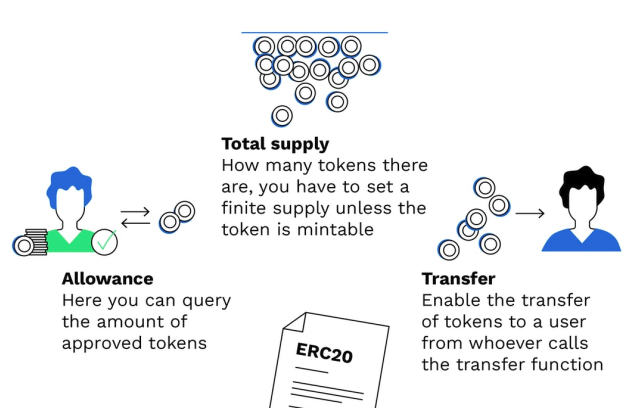
\includegraphics[scale=0.4,clip=false]{pictures/erc20_1.png}
  \end{center}
  
\end{frame}

\begin{frame}\frametitle{ERC20 Tokens}

  \begin{center}
    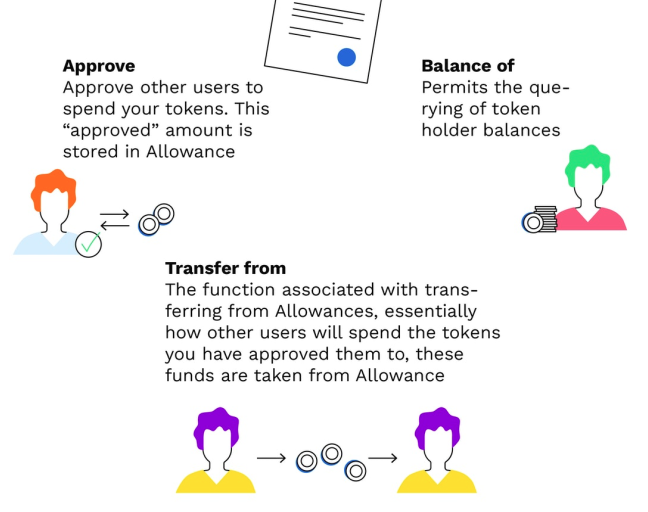
\includegraphics[scale=0.4,clip=false]{pictures/erc20_2.png}
  \end{center}
  
\end{frame}

\begin{frame}\frametitle{There are many\ldots}

  \begin{center}
    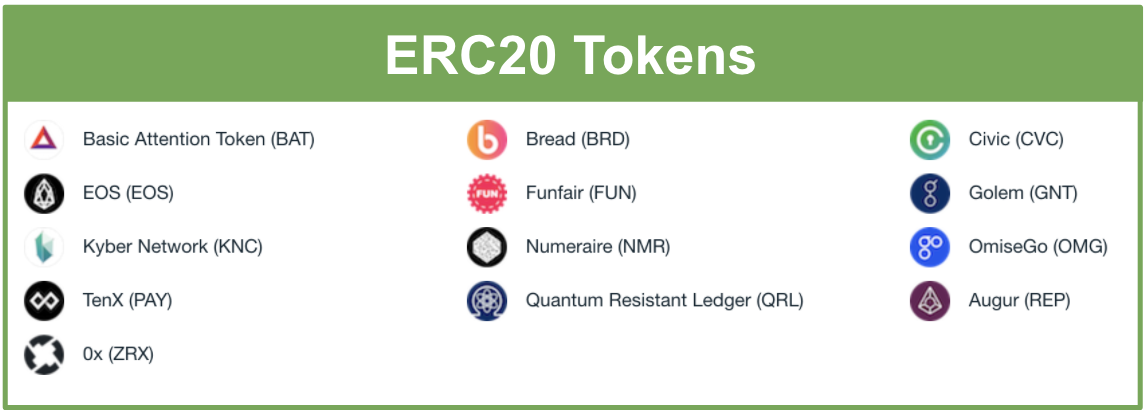
\includegraphics[scale=0.3,clip=false]{pictures/ERC20s.png}
  \end{center}
  
\end{frame}

\begin{frame}\frametitle{The OpenZeppelin reference implementation}

  \begin{greenbox}{We follow (in part) the implementation by OpenZeppelin}
    \begin{center}
      
\includegraphics[scale=0.2,clip=false]{pictures/open-zeppelin.jpg}
    \end{center}
    \begin{center}
      \url{https://docs.openzeppelin.com/contracts/2.x/api/token/erc20}
    \end{center}
  \end{greenbox}
  
\end{frame}

\begin{frame}\frametitle{The hierarchy of the implementation$^*$}

  \vspace*{-3ex}
  \begin{center}
    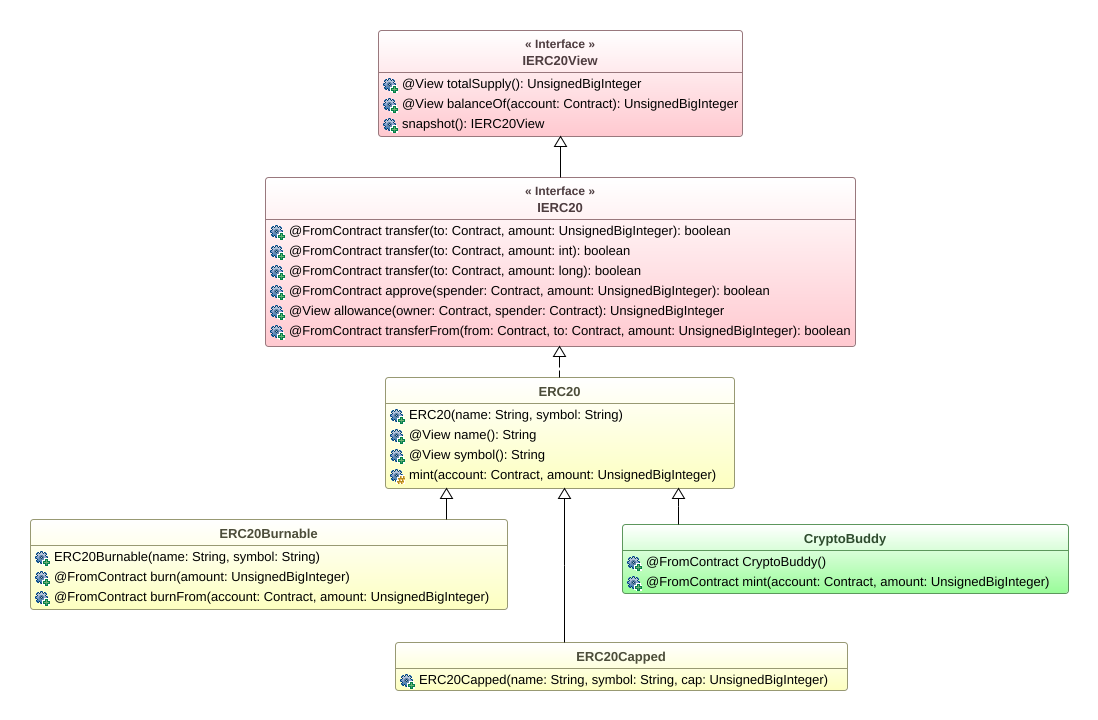
\includegraphics[scale=0.4,clip=false]{pictures/erc20-uml.png}
  \end{center}

  \vspace*{-2ex}
  {\tiny $^*$ Joint work with Marco Crosara}

\end{frame}

\begin{frame}[fragile]\frametitle{The \<IERC20View> interface}

  \begin{greenbox}{}
    This interface represents the read-only part of the standard.
    It allows one to create a \alert{snaphot} of a token, that is,
    a fixed, immutable snapshot of its balances
  \end{greenbox}

  \bigskip

  \begin{semiverbatim}
public interface IERC20View \{
  {\color{red}@View} UnsignedBigInteger totalSupply();
  {\color{red}@View} UnsignedBigInteger balanceOf(Contract account);
  IERC20View snapshot(); // not in OpenZeppelin
\}
  \end{semiverbatim}

\end{frame}

\begin{frame}[fragile]\frametitle{The \<IERC20> interface}

  \begin{greenbox}{}
    This interface represents the transfer part of the standard.
    Methods that require to identify their caller are
    annotated as {\color{red}\<@FromContract>}
  \end{greenbox}

  \smallskip

  {\scriptsize\begin{semiverbatim}
public interface IERC20 {\color{red}extends IERC20View} \{
  {\color{red}@FromContract} boolean transfer(Contract recipient, UnsignedBigInteger amount);
  {\color{red}@View} UnsignedBigInteger allowance(Contract owner, Contract spender);
  {\color{red}@FromContract} boolean approve(Contract spender, UnsignedBigInteger amount);
  {\color{red}@FromContract} boolean transferFrom
      (Contract sender, Contract recipient, UnsignedBigInteger amount);

  class Transfer {\color{red}extends Event} \{
    public final Contract from, to;
    public final UnsignedBigInteger value;

    {\color{red}@FromContract} Transfer(Contract from, Contract to, UnsignedBigInteger value) \{
      this.from = from;
      this.to = to;
      this.value = value;
    \}
  \}
\}
  \end{semiverbatim}}

\end{frame}

\begin{frame}[fragile]\frametitle{The \<ERC20> implementation: state}

{\scriptsize\begin{semiverbatim}
public class ERC20 {\color{red}extends Contract implements IERC20} \{
  {\color{violet}private final StorageMap<Contract, UnsignedBigInteger>
    balances = new StorageTreeMap<>();}

  {\color{blue}private final StorageMap<Contract, StorageMap<Contract, UnsignedBigInteger>>
    allowances = new StorageTreeMap<>();}

  public final UnsignedBigInteger ZERO = new UnsignedBigInteger("0");

  // there are public accessors to these fields (not shown)
  private UnsignedBigInteger totalSupply = ZERO;
  private final String name;
  private final String symbol;
  private short decimals;

  public ERC20(String name, String symbol) \{
    this.name = name;
    this.symbol = symbol;
    this.decimals = 18;
  \}
\}
\end{semiverbatim}}

\end{frame}

\begin{frame}[fragile]\frametitle{The \<ERC20> implementation: minting}

{\scriptsize\begin{semiverbatim}
public class ERC20 {\color{red}extends Contract implements IERC20} \{

  public final {\color{red}@View} UnsignedBigInteger balanceOf(Contract account) \{
    return balances.getOrDefault(account, ZERO);
  \}

  protected void _mint(Contract account, UnsignedBigInteger amount) \{
    {\color{armygreen}require(account != null, "Mint rejected: mint to the null account");
    require(amount != null, "Mint rejected: amount cannot be null");}

    beforeTokenTransfer(null, account, amount);
    totalSupply = totalSupply.add(amount);
    balances.put(account, balanceOf(account).add(amount));
  \}

  protected void beforeTokenTransfer
      (Contract from, Contract to, UnsignedBigInteger amount) \{ \}
\}
\end{semiverbatim}}

\end{frame}

\begin{frame}[fragile]\frametitle{The \<ERC20> implementation: transfer}

{\scriptsize\begin{semiverbatim}
public class ERC20 {\color{red}extends Contract implements IERC20} \{

  public {\color{red}@FromContract} boolean transfer(Contract to, UnsignedBigInteger amount) \{
    transfer(caller(), to, amount);
    return true;
  \}

  protected void transfer(Contract from, Contract to, UnsignedBigInteger amount) \{
    {\color{armygreen}require(from != null, "Transfer rejected: transfer from the null account");
    require(to != null, "Transfer rejected: transfer to the null account");
    require(amount != null, "Transfer rejected: amount cannot be null");}

    beforeTokenTransfer(from, to, amount);
    balances.put(from, balancesOf(from).subtract(amount,
      {\color{armygreen}"Transfer rejected: transfer amount exceeds balance"}));
    balances.put(to, balanceOf(to).add(amount));
    {\color{red}event(new Transfer(from, to, amount));}
  \}
\}
\end{semiverbatim}}

\end{frame}

\begin{frame}[fragile]\frametitle{The \<ERC20> implementation: approval}

{\scriptsize\begin{semiverbatim}
public class ERC20 {\color{red}extends Contract implements IERC20} \{

  public {\color{red}@View} UnsignedBigInteger allowance(Contract owner, Contract spender) \{
    return _allowances.getOrDefault(owner, StorageTreeMap::new)
                           .getOrDefault(spender, ZERO);
  \}

  public {\color{red}@FromContract} boolean approve(Contract spender, UnsignedBigInteger amount) \{
    approve(caller(), spender, amount);
    return true;
  \}

  protected void approve(Contract owner, Contract spender, UnsignedBigInteger amount) \{
    {\color{armygreen}require(owner != null, "Approve rejected: approve from the null account");
    require(spender != null, "Approve rejected: approve to the null account");
    require(amount != null, "Approve rejected: amount cannot be null");}

    StorageMap<Contract, UnsignedBigInteger> ownerAllowances
      = allowances.getOrDefault(owner, StorageTreeMap::new);
    ownerAllowances.put(spender, amount);
    allowances.put(owner, ownerAllowances);
    {\color{red}event(new Approval(owner, spender, amount));}
  \}
\}
\end{semiverbatim}}

\end{frame}

\begin{frame}[fragile]\frametitle{The \<ERC20> implementation: transfer from}

{\scriptsize\begin{semiverbatim}
public class ERC20 {\color{red}extends Contract implements IERC20} \{

  public {\color{red}@FromContract} boolean transferFrom
            (Contract from, Contract to, UnsignedBigInteger amount) \{

    transferFrom(caller(), from, to, amount);
    return true;
  \}

  protected final void transferFrom
        (Contract caller, Contract from, Contract to, UnsignedBigInteger amount) \{

    transfer(from, to, amount);
    approve(from, caller, allowance(from, caller).subtract(amount,
      {\color{armygreen}"Transfer Rejected: transfer amount exceeds allowance"}));
  \}
\}
\end{semiverbatim}}

\end{frame}

\begin{frame}\frametitle{Inconsistent view}

  \begin{center}
    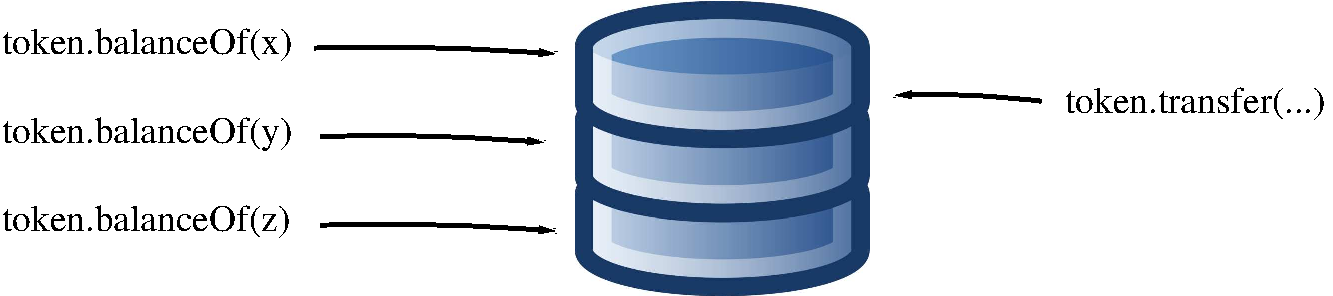
\includegraphics[scale=0.5,clip=false]{pictures/inconsistency.pdf}
  \end{center}

  \bigskip

  Between a call to \<balanceOf> and the next, the state of the token might change in the database
  because other users might call the transfer functions, concurrently

\end{frame}

\begin{frame}\frametitle{The view/snapshot design pattern}

  \begin{center}
    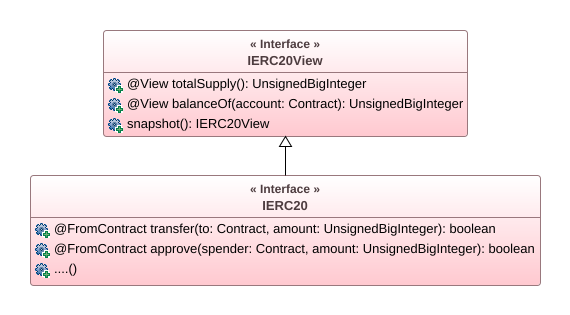
\includegraphics[scale=0.55,clip=false]{pictures/erc20-simplified-uml.png}
  \end{center}

  \begin{greenbox}{}
    An external wallet calls \<snapshot()> to get a consistent, immutable view of
    the token and can then access its content, while other clients can
    modify the original token
    \begin{itemize}
    \item impossible in Solidity, where maps cannot be cloned
    \end{itemize}
  \end{greenbox}

\end{frame}

\begin{frame}\frametitle{Inconsistent view}

  \begin{center}
    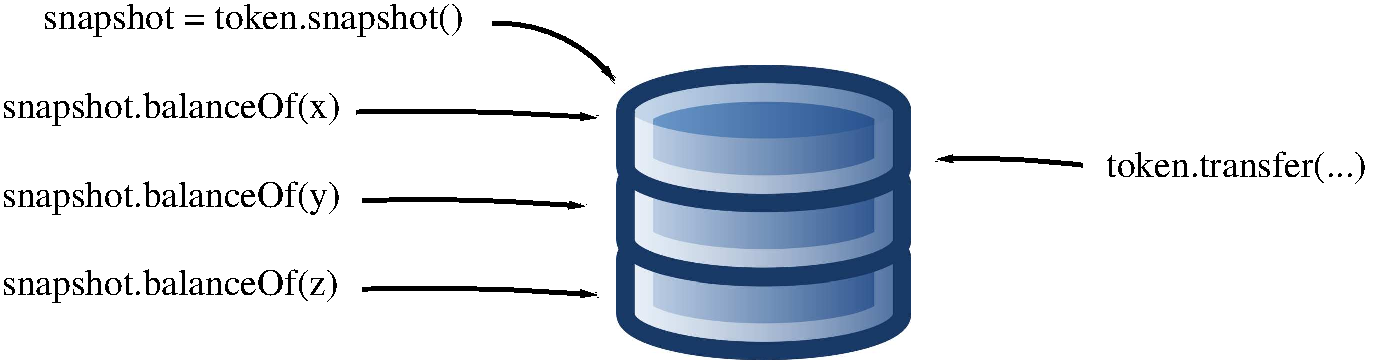
\includegraphics[scale=0.5,clip=false]{pictures/consistency.pdf}
  \end{center}

  \bigskip

  \begin{itemize}
  \item all calls to \<balanceOf> refer to the same, consistent state of the token (possibly not the
    latest)
  \item the implementation might keep a snapshot and provide a \<@View> method
    to read it
  \end{itemize}

\end{frame}

\begin{frame}[fragile]\frametitle{The \<ERC20> implementation: snapshot in O(1)}

\vspace*{-2ex}
{\scriptsize\begin{semiverbatim}
public class ERC20 {\color{red}extends Contract implements IERC20} \{

  public IERC20View snapshot() \{   {\color{violet}// O(1)}

    {\color{blue}class SnapshotImpl {\color{red}extends Storage implements IERC20View} \{
      private final UnsignedBigInteger totalSupply = ERC20.this.totalSupply;
      private final StorageMapView<Contract, UnsignedBigInteger> balances
        = ERC20.this.balances.snapshot(); {\color{violet}// O(1)}

      public {\color{red}@View} UnsignedBigInteger totalSupply() \{
        return totalSupply;
      \}

      public {\color{red}@View} UnsignedBigInteger balanceOf(Contract account) \{
        return balances.getOrDefault(account, ZERO);
      \}

      public IERC20View snapshot() \{
        return this; {\color{violet}// a snapshot of a snapshot is the snapshot itself}
      \}
    \}}

    return new SnapshotImpl();
  \}
\}
\end{semiverbatim}}

\end{frame}

\begin{frame}[fragile]\frametitle{Definition of a new token}

{\scriptsize\begin{semiverbatim}
public class {\color{red}CryptoBuddy extends ERC20} \{
  private final Contract owner;

  public {\color{red}@FromContract} CryptoBuddy() \{
    super("CryptoBuddy", "CB");

    owner = caller();
    UnsignedBigInteger initialSupply = new UnsignedBigInteger("200000");
    UnsignedBigInteger multiplier = new UnsignedBigInteger("10").pow(18);
    _mint(caller(), initialSupply.multiply(multiplier)); // 200'000 * 10 ^ 18
  \}

  public @FromContract void mintFor(Contract account, UnsignedBigInteger amount) \{
    require(caller() == owner, {\color{armygreen}"Lack of permission"});
    _mint(account, amount);
  \}
\}
\end{semiverbatim}}

\end{frame}

\begin{frame}\frametitle{Exercise}

  \begin{greenbox}{Define your own token}
  \begin{enumerate}
  \item implement the token in Takamaka (possibly using Eclipse or similar IDE)
  \item generate the jar of your new token
  \item use the Hotmoka Moka to install the jar in blockchain
  \item use the Hotmoka Moka to instantiate the token
  \item use the Hotmoka Moka to interact with the token
  \end{enumerate}
  \end{greenbox}

  \bigskip

  \begin{center}
    
\includegraphics[scale=0.12,clip=false]{pictures/tokens.png}
  \end{center}

\end{frame}

\begin{frame}\frametitle{A shared entity contract for governance}

  \begin{center}
    
\includegraphics[scale=0.38,clip=false]{pictures/shares.jpg}
  \end{center}

  \begin{itemize}
  \item the entity is initially split among \alert{shareholders},
    each in general holding a distinct number of \alert{shares}
  \item a shareholder can \alert{place an offer} to sell some or all of its shares
  \item a buyer can \alert{accept} an offer and become a shareholder
  \end{itemize}

\end{frame}

\begin{frame}\frametitle{The hierarchy of the implementation$^*$}

  \begin{center}
    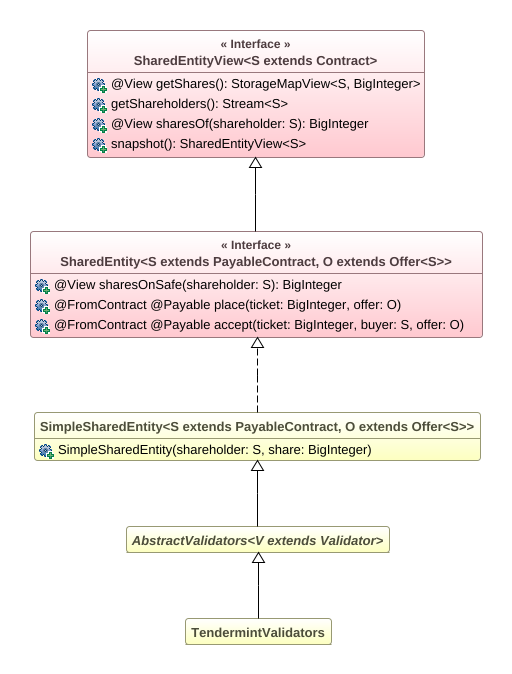
\includegraphics[scale=0.41,clip=false]{pictures/shared-entities-uml.png}
  \end{center}

  \vspace*{-3ex}
  {\tiny $^*$ Joint work with Andrea Benini}

\end{frame}

\begin{frame}[fragile]\frametitle{The \<SharedEntityView> interface}

  \begin{semiverbatim}
public interface {\color{red}SharedEntityView<S extends Contract>} \{
  {\color{red}@View} StorageMapView<S, BigInteger> getShares();
  Stream<S> getShareholders();
  {\color{red}@View} BigInteger sharesOf(S shareholder);
  SharedEntityView<S> snapshot();
\}
  \end{semiverbatim}

  \bigskip

  Note: generic types do not exist in Solidity

\end{frame}

\begin{frame}[fragile]\frametitle{The \<SharedEntity> interface: adds a market of shares}

  {\scriptsize\begin{semiverbatim}
public interface {\color{red}SharedEntity<S extends PayableContract, O extends Offer<S>>
    extends SharedEntityView<S>} \{

  {\color{red}@View} BigInteger sharesOnSaleOf(S shareholder);

  {\color{red}@FromContract @Payable} void place(BigInteger ticket, O offer);

  {\color{red}@FromContract @Payable} void accept(BigInteger ticket, S buyer, O offer);
\}
  \end{semiverbatim}}

  \begin{itemize}
  \item who sells its shares receives a payment: hence \<S> is constrained
    to extend \<PayableContract>
  \item Java does not allow one to write \<@FromContract(S.class)>
  \item the interface allows implementations to ask for a ticket when offers
    are placed and accepted
  \end{itemize}

\end{frame}

\begin{frame}[fragile]\frametitle{The \<Offer> inner class of \<SharedEntity>}

  {\tiny\begin{semiverbatim}
public static class {\color{red}Offer<S extends PayableContract>} extends Storage \{
  public final S seller;
  public final BigInteger sharesOnSale;
  public final BigInteger cost;
  public final long expiration;

  public {\color{red}@FromContract} Offer(S seller, BigInteger sharesOnSale, BigInteger cost, long duration) \{
    {\color{armygreen}require(caller() == seller, "only the owner can sell its shares");
    require(sharesOnSale != null && sharesOnSale.signum() > 0, "the shares on sale must be positive");
    require(cost != null && cost.signum() >= 0, "the cost must be a non-negative big integer");
    require(duration >= 0, "the duration cannot be negative");}

    this.seller = seller;
    this.sharesOnSale = sharesOnSale;
    this.cost = cost;
    this.expiration = now() + duration;
  \}

  public {\color{red}@View} boolean isOngoing() \{
    return now() <= expiration;
  \}
\}
  \end{semiverbatim}}

\end{frame}

\begin{frame}[fragile]\frametitle{The \<SimpleSharedEntity> implementation: state}

  {\scriptsize\begin{semiverbatim}
public class {\color{red}SimpleSharedEntity<S extends PayableContract, O extends Offer<S>>
      extends PayableContract implements SharedEntity<S, O>} \{

  private final StorageTreeMap<S, BigInteger> shares = new StorageTreeMap<>();
  private final StorageSet<O> offers = new StorageTreeSet<>();
  private StorageMapView<S, BigInteger> snapshotOfShares;

  public SimpleSharedEntity(S shareholder, BigInteger share) \{ // simple case
    shares.put(shareholder, share);
    snapshotOfShares = shares.snapshot();
  \}

  public {\color{red}@View} final StorageMapView<S, BigInteger> getShares() \{
    return snapshotOfShares;
  \}

  public final Stream<S> getShareholders() \{
    return snapshotOfShares.keys();
  \}

  public final {\color{red}@View} BigInteger sharesOf(S shareholder) \{
    return snapshotOfShares.getOrDefault(shareholder, ZERO);
  \}
\}
  \end{semiverbatim}}

\end{frame}

\begin{frame}[fragile]\frametitle{The \<SimpleSharedEntity> implementation: shares on sale}

  \textit{Add the shares on sale of every offer placed by the shareholder
  and still ongoing}

\bigskip

{\scriptsize\begin{semiverbatim}
public final {\color{red}@View} BigInteger sharesOnSaleOf(S shareholder) \{
  return offers.stream()
    .filter(offer -> offer.seller == shareholder && offer.isOngoing())
    .map(offer -> offer.sharesOnSale)
    .reduce(ZERO, BigInteger::add);
\}
  \end{semiverbatim}}

\end{frame}

\begin{frame}[fragile]\frametitle{The \<SimpleSharedEntity> implementation: place an offer}

  \textit{If the offer is valid, add it to the set of offers, removing expired offers on the way}

\bigskip

{\scriptsize\begin{semiverbatim}
public {\color{red}@FromContract @Payable} void place(BigInteger ticket, O offer) \{
  {\color{armygreen}require(offer.seller == caller(), "only the seller can place its own offer");
  require(shares.containsKey(offer.seller), "the seller is not a shareholder");
  require(sharesOf(offer.seller).subtract(sharesOnSaleOf(offer.seller))
    .compareTo(offer.sharesOnSale) >= 0, "the seller has not enough shares");}
  cleanUpOffers(null);
  offers.add(offer);
\}

private void cleanUpOffers(O offerToRemove) \{
  offers.stream()
    .filter(offer -> offer == offerToRemove || !offer.isOngoing())
    .forEachOrdered(offers::remove);
\}
\end{semiverbatim}}

\end{frame}

\begin{frame}[fragile]\frametitle{The \<SimpleSharedEntity> implementation: accept an offer}

  \textit{If the offer is valid, remove it, swap the shares and send the payment to the seller}

\bigskip

{\scriptsize\begin{semiverbatim}
public {\color{red}@FromContract @Payable} void accept(BigInteger ticket, S buyer, O offer) \{
  {\color{armygreen}require(caller() == buyer, "only the future owner can buy the shares");
  require(offers.contains(offer), "unknown offer");
  require(offer.isOngoing(), "the sale offer is not ongoing anymore");
  require(offer.cost.compareTo(ticket) <= 0, "not enough money for the offer");}
  cleanUpOffers(offer);
  removeShares(offer.seller, offer.sharesOnSale);
  addShares(buyer, offer.sharesOnSale);
  offer.seller.receive(offer.cost);
  snapshotOfShares = shares.snapshot();
\}

private void addShares(S shareholder, BigInteger added) \{
  shares.update(shareholder, BigInteger.ZERO, added::add);
\}

private void removeShares(S shareholder, BigInteger removed) \{
  ... similar
\}
\end{semiverbatim}}

\end{frame}

\begin{frame}[fragile]\frametitle{The \<SimpleSharedEntity> implementation: snapshot}

  \textit{Save the current snapshot of the shares, to answer all questions}

\medskip

{\scriptsize\begin{semiverbatim}
public final SharedEntityView<S> snapshot() \{

  {\color{blue}class SharedEntitySnapshotImpl implements SharedEntityView<S> \{
    {\color{red}private final StorageMapView<S, BigInteger> snapshotOfShares
        = SimpleSharedEntity.this.snapshotOfShares;}

    public StorageMapView<S, BigInteger> getShares() \{ return snapshotOfShares; \}

    public Stream<S> getShareholders() \{
      return snapshotOfShares.keys();
    \}

    public BigInteger sharesOf(S shareholder) \{
      return snapshotOfShares.getOrDefault(shareholder, ZERO);
    \}

    public SharedEntityView<S> snapshot() \{ return this; \}
  \};}

  return new SharedEntitySnapshotImpl();
\}
\end{semiverbatim}}

\end{frame}

\begin{frame}\frametitle{Exercise}

  \begin{greenbox}{Define a lottery contract}
  \begin{enumerate}
  \item the creator (a payable contract)
    specifies, at the lottery creation time, the number $N\ge 2$ of tickets to sell
  \item payable contracts can call a \<void buy()> method of the lottery to buy a ticket
    (possibly many times). The ticket costs $100000\cdot\left(1 + \frac{\text{number of tickets already sold}}{N-1}\right)$
  \item when the $N$th ticket is sold, the method \<buy> computes \<now() \% N> and determines
    the number of the winning contract
    \begin{itemize}
    \item it sends $90\%$ of the balance of the lottery to the winner
    \item it sends the remaining $10\%$ of the balance of the lottery to its creator
    \item it rejects all future calls to \<buy>
    \end{itemize}
  \item install the contract in blockchain and play with it by using the Moka
  \end{enumerate}
  \end{greenbox}

  \medskip

  Suggestion: keep the ticket holders inside a \<io.takamaka.code.util.StorageLinkedList> field
  (from the Takamaka library)
\end{frame}

\end{document}
